\documentclass{article}

\usepackage[margin=1in]{geometry}
\usepackage{amsmath,amssymb}
\usepackage{dsfont}
\usepackage{tikz}
\usetikzlibrary{bayesnet}

\author{Otto Fabius}
\title{SGVB Topic Modelling}
\begin{document}

\maketitle

\section{Model}

We will consider the following graphical model:

\begin{figure}[ht]
  \begin{center}
    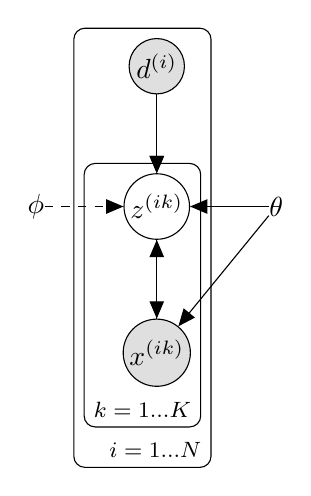
\begin{tikzpicture}[node distance = 1.5cm]
        \node[obs] (x) {$x^{(ik)}$}; 

        \node[latent, above=of x] (z) {$z^{(ik)}$}; 
        
        \node[obs, above=of z] (d) {$d^{(i)}$}; 

        \node[const, right=of z] (th) {$\theta$} ;
        \node[const, left=of z] (ph) {$\phi$};

        \edge {z} {x};
        \edge {d} {z};
        \edge {th} {z};
        \edge {th} {x};

        \edge [dashed] {ph} {z}
        \edge [dashed,bend right] {d} {z}
        \edge [dashed,bend left] {x} {z}
		
		\plate {xz} {(x)(z)} {$k = 1...K$};
        \plate {xzd} {(x)(z)(d)(xz)} {$i = 1...N$};

    \end{tikzpicture}
  \end{center}
\caption{Graphical Model}
\label{sgvb}
\end{figure}

In our application, $\mathbf{d}^{(i)}$ is a document (a vector of word frequencies), selected from the dataset containing N documents with uniform probability. The number of words in a document is K so $\mathbf{x}^{(ik)}$ is a word in $\mathbf{d}^{(i)}$, with $p(\mathbf{x}^{(ik)}|\mathbf{z}^{(ik)})$ a multinomial distribution. The (continuous) latent variables $\mathbf{z}^{(ik)}$ represent the topic, with $p(\mathbf{z}^{(ik)}|\mathbf{d}^{(i)})$ a multivariate normal distribution with diagonal covariance. We have a separate $\mathbf{z}^{(ik)}$ for each word $\mathbf{x}^{(ik)}$ in $\mathbf{d}^{(i)}$.\\ \\
We approximate the true posterior $p(z|x,d)$ by $q_\phi(z|x,d)$ parametrized by $\phi$, once again a multivariate normal distribution with diagonal covariance. All three the distributions $p_\theta(z|d)$, $p_\theta(x|z)$, and $q_\phi(z|x,d)$ are neural networks, of which the parameters $\theta$ and $\phi$ are to be learned jointly. The output of $p_\theta(z|d)$ and $q_\phi(z|x,d)$ are the mean and the diagonal entries of the covariance matrix.\\ 

The network $q_\phi(z|x,d)$ has as input $x^{(ik)}$ and $d^{(i)}$. It makes sense to have at least one separate hidden layer for $d^{(i)}$ and $x^{(ik)}$ as both are very sparse and can be represented in lower-dimensional space. Furthermore, the hidden representation of $d^{(i)}$ may only have to be computed once for all $k$ words $x^{(ik)}$ in $d^{(i)}$.

\section{Math}

\subsection{Lower Bound}

The log-likelihood of a data point i can be written as a sum of the lower bound and the KL divergence term between the true posterior $p(z|x,d)$ and the approximation $q(z|x,d)$, with $\theta$ the parameters of the model:

\begin{align*}
    \log p(\mathbf{x}^{(ik)}) = D_{KL}(q(\mathbf{z}|\mathbf{x}^{(ik)},\mathbf{d}^{(i)}) || p(\mathbf{z}|\mathbf{x}^{(ik)},\mathbf{d}^{(i)})) + \mathcal{L}(\mathbf{\theta}, \phi; \mathbf{x}^{(ik)})
\end{align*}

We try to optimize the lowerbound: 

\begin{align}
\mathcal{L}(\mathbf{\theta}, \phi; \mathbf{x}^{(ik)}, \mathbf{d}^{(i)}) = \mathds{E}_{q_\phi(\mathbf{z}|\mathbf{x}^{ik},\mathbf{d}^{i})}[-\log q_\phi (\mathbf{z}| \mathbf{x}^{(ik)}, \mathbf{d}^{(i)})+\log p_\theta(\mathbf{z}, \mathbf{x}^{(ik)}|\mathbf{d}^{(i)} ]
\end{align}

which, using Bayes rule, we can express as:

\begin{align}
\mathcal{L}(\mathbf{\theta}, \phi; \mathbf{x}^{(ik)}, \mathbf{d}^{(i)}) = -D_{KL}(q_\phi (\mathbf{z}| \mathbf{x}^{(ik)}, \mathbf{d}^{(i)})||q_\phi (\mathbf{z}| \mathbf{d}^{(i)})) + \mathds{E}_{q_\phi(\mathbf{z}|\mathbf{x}^{(ik)},\mathbf{d}^{(i)})}[\log p_\theta (\mathbf{x}^{(ik)}|\mathbf{z})]
\end{align}

Note that in the last term we don't condition on $\mathbf{d}^{(i)}$: $\mathbf{x}^{(ik)}$ is conditionally independent of $\mathbf{d}^{(i)}$ in our model.

\subsection{KL Divergence}

We can integrate the KL divergence analytically. We don't use indices $^{(ik)}$ for this integral. Further, $\mathbf{\mu}_\theta$ and $\mathbf{\sigma}_\theta^2$ represent the parametrized $p(\mathbf{z}|\mathbf{d})$ and $\mathbf{\mu}_\phi$ and $\mathbf{\sigma}_\phi^2$ represent the parametrized $p(\mathbf{z}|\mathbf{x},\mathbf{d})$ (both are multivariate normals with diagonal covariance).

\begin{align}
D_{KL}(q_\phi (\mathbf{z}| \mathbf{x}, \mathbf{d}||p_\theta (\mathbf{z}| \mathbf{d})) =
\int(q_\phi (\mathbf{z}| \mathbf{x}, \mathbf{d})\log \frac{q_\phi (\mathbf{z}| \mathbf{x}, \mathbf{d})}{p_\theta (\mathbf{z}| \mathbf{d})})d\mathbf{z}
\end{align}

%\begin{align}= \int\{ \mathcal{N}(\mathbf{z};\mathbf{\mu_\phi},\mathbf{\sigma_\phi}^2\mathbf{I}) ( \log \mathcal{N}(\mathbf{z};\mathbf{\mu_\phi},\mathbf{\sigma_\phi}^2\mathbf{I}) - \log \mathcal{N}(\mathbf{z};\mathbf{\mu_\theta},\mathbf{\sigma_\theta}^2 \mathbf{I}))\}d\mathbf{z}\end{align}

Following the general solution for KLD between two multivariate normals we obtain:

\begin{align}
D_{KL}(q_\phi (\mathbf{z}| \mathbf{x}, \mathbf{d}||p_\theta (\mathbf{z}| \mathbf{d})) = \frac{1}{2}\{Tr((\sigma_\theta^2\mathbf{I})^{-1}(\sigma_\phi^2\mathbf{I})) + (\mu_\phi - \mu_\theta)^T(\sigma_\theta^2\mathbf{I})^{-1}(\mu_\phi - \mu_\theta) - \log\frac{(\sigma_\phi^2\mathbf{I})}{(\sigma_\theta^2\mathbf{I})} - J\}
\end{align}
Where the squares of the vectors $\sigma_\phi$ and $\sigma_\theta$ are element-wise. We have diagonal covariance, so we can simplify a bunch:

\begin{align}
D_{KL}(q_\phi (\mathbf{z}| \mathbf{x}, \mathbf{d})||p_\theta (\mathbf{z}| \mathbf{d})) = \frac{1}{2}\sum\limits_{j=1}^{J}\{\frac{\sigma_{\phi,j}^2}{\sigma_{\theta,j}^2} + \frac{(\mu_{\phi,j} - \mu_{\theta,j})^2}{\sigma_{\theta,j}^2} + \log \sigma_{\theta,j}^2 - \log \sigma_{\phi,j}^2 - 1\}
\end{align}

\subsection{SGVB estimator}

For the second part of the lower bound, $\mathds{E}_{q_\phi(\mathbf{z}|\mathbf{x}^{(ik)},\mathbf{d}^{(i)})}[\log p_\theta (\mathbf{x}^{(ik)}|\mathbf{z})]$, we use a reparametrization of $\mathbf{z}$:

\begin{align} \mathbf{z}^{(ik)} = g_\phi(\mathbf{\epsilon}^{(ik)}, \mathbf{x}^{(ik)}) \text{    and    } \mathbf{\epsilon} 
 \sim p(\mathbf{\epsilon}) \text{   with  } p(\epsilon) = \mathcal{N}(\epsilon|0,1)
\end{align}

Note that we use only one sample of $\mathbf{z}^{(ik)}$ here (i.e. L=1 in Kingma \& Welling 2013), which we know works well if we use batches ($>100$) during optimization.

Our estimator of the second part is now $\log p_\theta (\mathbf{x}^{(ik)}|\mathbf{z}^{(ik)})$, which is a multinomial. We use a softmax in the final layer to output $\mathbf{y}^{(ik)}$, which represents the word probabilities, to ensure that $\sum\limits_{j=1}^J y_j^{(ik)} = 1$. The log likelihood becomes: 

\begin{align}
\log p_\theta (\mathbf{x}^{(ik)}|\mathbf{z}^(ik)) = \sum\limits_{j=1}^{J}x_j^{(ik)}\log y_j^{(ik)}
\end{align}

\subsection{Final objective function}

$\mathcal{L}(\mathbf{\theta}, \phi; \mathbf{x}^{(i)}, \mathbf{d}^{(i)}) = - \frac{1}{2}\sum\limits_{j=1}^{J}\{\frac{\sigma_{\phi,j}^2}{\sigma_{\theta,j}^2} + \frac{(\mu_{\phi,j} - \mu_{\theta,j})^2}{\sigma_{\phi,j}^2} + \log \sigma_{\theta,j}^2 - \log \sigma_{\phi,j}^2 - 1 - x_j^{(i)}\log d_j^{(i)} \}$

\end{document}